%%%%%%%%%%%%%%%%%%%%%%%%%%%%%%%%%%%%%%%%%%%%%%%
\chapter{Combinatorial Results} \label{chap:comb_res}
%%%%%%%%%%%%%%%%%%%%%%%%%%%%%%%%%%%%%%%%%%%%%%%

In previous studies \cite{Wachter-Zeh:2018}, there was no general
vector solution found for multicast networks with $h=3$ messages.
Hence, we start with a probabilistic argument to prove that there
exists a vector solution outperforming the optimal linear solution
for the $\left(\epsilon=1,l=1\right)-\mathcal{N}_{h=3,r,s=4}$ network.
Then we generalize the proof to the $\left(\epsilon=1,l=1\right)-\mathcal{N}_{h,r,s}$
network.

\section{$\left(\epsilon=1,l=1\right)-\mathcal{N}_{h=3,r,s=4}$ Network \label{sec:Network_e1l1h3rs4}}

\begin{figure}[H]
\caption{The $(\epsilon=1,l=1)-\mathcal{N}_{h=3,r,s=4}$ network\label{fig:nw_e1_l1_h3_r_s4}}

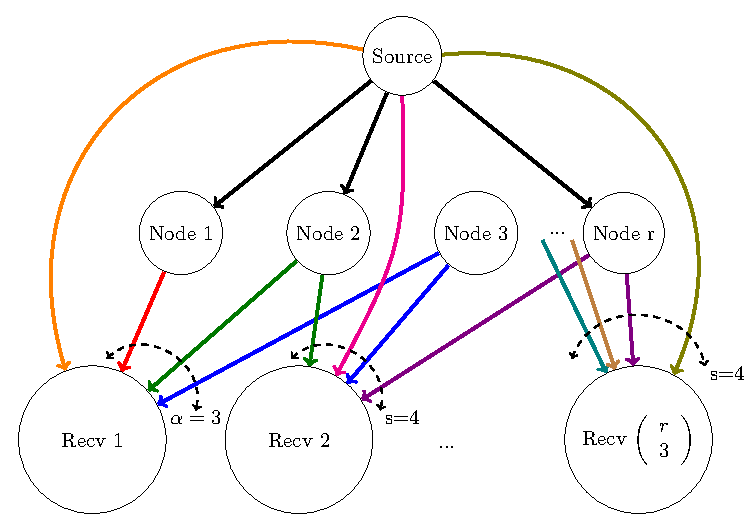
\includegraphics[width=0.5\paperwidth]{E:/Documents/TUM/THESIS/thesisCOD_Ha/figures/nw_e1_l1_h3_r_s4}
\end{figure}

In this subsection, we derive a lower bound on the number of receivers
for the $\left(\epsilon=1,l=1\right)-\mathcal{N}_{h=3,r,s=4}$ network.
Due to $\alpha=3$, the number of receivers is $N=\left(\begin{array}{c}
r_{vector}\\
3
\end{array}\right)$ by definition in Section \ref{sec:Description_GCN}. To derive the
lower bound, we introduce a rank requirement on incoming packets to
each receiver. 

\begin{figure}[H]
\caption{The vector network coding of $(\epsilon=1,l=1)-\mathcal{N}_{h=3,r,s=4}$
represents as a matrix problem\label{fig:rk_h3}}

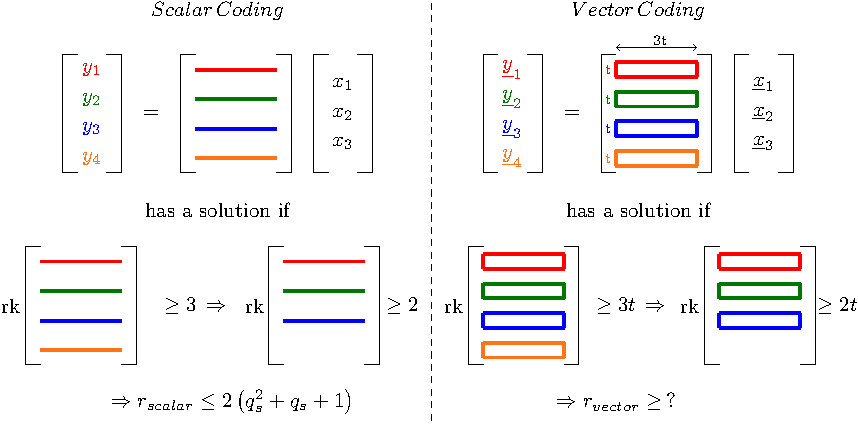
\includegraphics[width=0.5\paperwidth]{E:/Documents/TUM/THESIS/thesisCOD_Ha/figures/rk_h3}
\end{figure}

Following to Equation \ref{eq:linear_system}, each receiver must
solve a linear equation system of 3 variables with 4 equations to
recover $h=3$ messages as below:

\[
\left[\begin{array}{c}
\underline{y}_{j_{1}}\\
\underline{y}_{j_{2}}\\
\underline{y}_{j_{3}}\\
\underline{y}_{j_{4}}
\end{array}\right]=\boldsymbol{A}_{j}\cdot\underline{x}=\left[\begin{array}{c}
\boldsymbol{A}_{j_{1}}\\
\boldsymbol{A}_{j_{2}}\\
\boldsymbol{A}_{j_{3}}\\
\boldsymbol{A}_{j_{4}}
\end{array}\right]\cdot\left[\begin{array}{c}
\underline{x}_{1}\\
\underline{x}_{2}\\
\underline{x}_{3}
\end{array}\right],
\]

with $\underline{x}_{i},\underline{y}_{j_{v}}\in\ensuremath{\mathbb{F}}_{q}^{t},\boldsymbol{A}_{j_{v}}\in\ensuremath{\mathbb{F}}_{q}^{t\times3t}$
for $v=1,\ldots,4$, and $\boldsymbol{A}_{j_{1}},\ldots,\boldsymbol{A}_{j_{3}}$
must be distinct.

The network is solvable, if $\boldsymbol{A}_{j}$ has full-rank, i.e.
$\boldsymbol{A}_{j_{v}}$ must satisfy:

\[
rk\left[\begin{array}{c}
\boldsymbol{A}_{j_{1}}\\
\boldsymbol{A}_{j_{2}}\\
\boldsymbol{A}_{j_{3}}\\
\boldsymbol{A}_{j_{4}}
\end{array}\right]\geq3t
\]

In order to satisfy $rk\left[\boldsymbol{A}_{j}\right]\geq3t$, we
can easily choose suitable values for the coefficient $\boldsymbol{A}_{j_{4}}$
on the direct link from the source to $R_{j}$. However, the coefficients
on the links from nodes to receivers are matters. Therefore, we focus
on the following requirement:

\begin{equation}
rk\left[\begin{array}{c}
\boldsymbol{A}_{j_{1}}\\
\boldsymbol{A}_{j_{2}}\\
\boldsymbol{A}_{j_{3}}
\end{array}\right]\geq2t\label{eq:rk_rqm_e1l1h3s4}
\end{equation}

This means that $rk\left[\begin{array}{c}
\boldsymbol{A}_{j_{1}}\\
\boldsymbol{A}_{j_{2}}\\
\boldsymbol{A}_{j_{3}}
\end{array}\right]\geq2t$ implies $rk\left[\boldsymbol{A}_{j}\right]\geq3t$, or to satisfy
$rk\left[\boldsymbol{A}_{j}\right]\geq3t$, we need $rk\left[\begin{array}{c}
\boldsymbol{A}_{j_{1}}\\
\boldsymbol{A}_{j_{2}}\\
\boldsymbol{A}_{j_{3}}
\end{array}\right]\geq2t$.

By this constraint, the problem is thus described as below:

\[
\underset{rk\left[\boldsymbol{A}_{j}\right]\geq3t}{min}\,r_{vector}
\]

$\boldsymbol{A}_{j_{1}},\boldsymbol{A}_{j_{2}},\boldsymbol{A}_{j_{3}}$
are matrices formed on any 3 of $r$ links from nodes to receivers,
i.e. these 3 matrices are randomly chosen from a set of $r$ matrices.
We formalize the problem by an approach with Lov\'asz local lemma
\cite{MosheSchwartz:2018}.
\begin{lem}[Symmetric Lov\'asz local lemma (LLL)]
 \cite{Schwarz:2013} A set of events $\mathcal{E}_{i}$, with $i=1,\ldots,n$,
such that each event occurs with probability at most $p$. If each
event is independent of all others except for at most $d$ of them
and $4dp\leq1$, then: $Pr\left[\stackrel[i=1]{n}{\bigcap}\overline{\mathcal{E}}_{i}\right]>0$.
\label{thm:LLL}
\end{lem}
%
\begin{lem}
For the network $\left(\epsilon=1,l=1\right)-\mathcal{N}_{h=3,r,s=4}$,
the probability that vector solution does not exist is equal to $\frac{1}{q^{9t^{2}}}\stackrel[i=0]{2t-1}{\mathop{\sum}}\stackrel[j=0]{i-1}{\mathop{\prod}}\frac{\left(q^{3t}-q^{j}\right)^{2}}{q^{i}-q^{j}}$.
\label{lem:prob_p_LLL_formula}
\end{lem}
\textit{Proof}. For our problem, let $\mathcal{E}_{i}$ denote the
following event:

\[
Pr\left[\mathcal{E}_{i}\right]=Pr\left[rk\left[\begin{array}{c}
\boldsymbol{A}_{j_{1}}\\
\boldsymbol{A}_{j_{2}}\\
\boldsymbol{A}_{j_{3}}
\end{array}\right]<2t\right]
\]

Because the rank requirement in Equation \ref{eq:rk_rqm_e1l1h3s4}
is opposite, we consider the complement event $T$:

\[
rk\left[\begin{array}{c}
\boldsymbol{A}_{j_{1}}\\
\boldsymbol{A}_{j_{2}}\\
\boldsymbol{A}_{j_{3}}
\end{array}\right]\geq2t,\forall1\leq j_{1}<j_{2}<j_{3}\leq r
\]

By the intersection rule, we have:

\[
T=\underset{\mathcal{E}_{i}\in\mathcal{E}}{\bigcap}\overline{\mathcal{E}}_{i}
\]

The probability of event $T$ indicates a measure quantifying the
likelihood that we will be able to construct $rk\left[\boldsymbol{A}_{j}\right]\geq3t$
with $j_{1,}j_{2},j_{3}$ in the integer numbers between $1$ and
$r$, including both. We need to maximize $r$, and the rank requirement
\ref{eq:rk_rqm_e1l1h3s4} must be satisfied, i.e. the probabilty of
event $T$ must be higher than $0$:

\begin{eqnarray*}
 & Pr\left[rk\left[\begin{array}{c}
\boldsymbol{A}_{j_{1}}\\
\boldsymbol{A}_{j_{2}}\\
\boldsymbol{A}_{j_{3}}
\end{array}\right]\geq2t,\forall1\leq j_{1}<j_{2}<j_{3}\leq r\right] & >0\\
\Leftrightarrow & Pr\left[T\right] & >0\\
\Leftrightarrow & Pr\left[\underset{\mathcal{E}_{i}\in\mathcal{E}}{\bigcap}\overline{\mathcal{E}}_{i}\right] & >0
\end{eqnarray*}

Following to LLL, each event occurst with probability at most $p$:

\begin{equation}
Pr\left[\mathcal{E}_{i}\right]=Pr\left[rk\left[\begin{array}{c}
\boldsymbol{A}_{i_{1}}\\
\boldsymbol{A}_{i_{2}}\\
\boldsymbol{A}_{i_{3}}
\end{array}\right]<2t\right]\leq p\label{eq:p_in_LLL}
\end{equation}

Regarding to the left-hand side:

\begin{eqnarray}
Pr\left[rk\left[\begin{array}{c}
\boldsymbol{A}_{i_{1}}\\
\boldsymbol{A}_{i_{2}}\\
\boldsymbol{A}_{i_{3}}
\end{array}\right]<2t\right] & = & \stackrel[i=0]{2t-1}{\mathop{\sum}}Pr\left[rk\left[\begin{array}{c}
\boldsymbol{A}_{i_{1}}\\
\boldsymbol{A}_{i_{2}}\\
\boldsymbol{A}_{i_{3}}
\end{array}\right]=i\right]\nonumber \\
 & \overset{1}{=} & \stackrel[i=0]{2t-1}{\mathop{\sum}}\frac{N_{t,m,n}}{q^{m\cdot n}}\nonumber \\
 & = & \stackrel[i=0]{2t-1}{\mathop{\sum}}\frac{\stackrel[j=0]{i-1}{\mathop{\prod}}\frac{\left(q^{m}-q^{j}\right)\left(q^{n}-q^{j}\right)}{q^{i}-q^{j}}}{q^{m\cdot n}}\nonumber \\
 & \overset{2}{=} & \stackrel[i=0]{2t-1}{\mathop{\sum}}\frac{\stackrel[j=0]{i-1}{\mathop{\prod}}\frac{\left(q^{3t}-q^{j}\right)^{2}}{q^{i}-q^{j}}}{q^{9t^{2}}}\Square\label{eq:p_eq_h3}
\end{eqnarray}

By varying $t$ in Equation (\ref{eq:p_eq_h3}), we have the following
table:

\begin{table}[H]
\caption{$r$ over variations of t\label{tab:r_over_t}}

\begin{tabular}{|c|c|c|}
\hline 
t & Scalar Solution & Vector Solution\tabularnewline
\hline 
\hline 
1 & $r_{scalar}\leq14$ & $r_{vector}\geq3$\tabularnewline
\hline 
2 & $r_{scalar}\leq42$ & $r_{vector}\geq7\,\left(67^{*},\,89^{**}\right)$\tabularnewline
\hline 
3 & $r_{scalar}\leq146$ & $r_{vector}\geq62\,\left(166^{*}\right)$ \tabularnewline
\hline 
4 & $r_{scalar}\leq546$ & $r_{vector}\geq1317$\tabularnewline
\hline 
5 & $r_{scalar}\leq2114$ & $r_{vector}\geq58472$\tabularnewline
\hline 
6 & $r_{scalar}\leq8322$ & $r_{vector}>10^{6}$\tabularnewline
\hline 
\end{tabular}

{*}, {*}{*}: computational results in construction 1 and construction
2 respectively
\end{table}

In the table (\ref{tab:r_over_t}), the vector solution outperforms
the scalar solution when $t\geq4$ for the network $\left(\epsilon=1,l=1\right)-\ensuremath{N}_{h=3,r,s=4}$.
This is sufficient, later on we show computational results which vector
solutions outperform scalar solutions in case of $t=2$ and $t=3$.
\begin{lem}
For the network $\left(\epsilon=1,l=1\right)-\mathcal{N}_{h=3,r,s=4}$,
the probability that vector solution does not exist is less than or
equal to $\Theta\left(q^{-t^{2}-2t-1}\right)$. \label{lem:tight_bound_p}
\end{lem}
\textit{Proof}. This lemma is a tight bound for Equation \ref{eq:p_in_LLL}
in Lemma \ref{lem:prob_p_LLL_formula}, i.e. we try to maximize $p$
with an exact maximum value. We consider the nominator of Equation
(\ref{eq:p_eq_h3}):

\[
\stackrel[j=0]{i-1}{\mathop{\prod}}\frac{\left(q^{3t}-q^{j}\right)^{2}}{q^{i}-q^{j}}=\frac{p_{N}^{(i)}(q)}{p_{D}^{(i)}(q)}=p^{(i)}(q)
\]

Due to $i$-times product and large $t$:

\[
\left.\begin{array}{c}
deg\left(p_{N}^{(i)}(q)\right)=q^{i6t}\\
deg\left(p_{D}^{(i)}(q)\right)=q^{i^{2}}
\end{array}\right\} \Rightarrow p^{(i)}(q)\approx q^{i6t-i^{2}}
\]

Then we have:

\[
\stackrel[i=0]{2t-1}{\mathop{\sum}}\stackrel[j=0]{i-1}{\mathop{\prod}}\frac{\left(q^{3t}-q^{j}\right)^{2}}{q^{i}-q^{j}}=\stackrel[i=0]{2t-1}{\mathop{\sum}}p^{(i)}(q)\approx\stackrel[i=0]{2t-1}{\mathop{\sum}}q^{i6t-i^{2}}
\]

To maximize the sum, we set derivation of to 0 and find its root:

\begin{eqnarray*}
 & \left(i6t-i^{2}\right)^{'} & =0\\
\Leftrightarrow & 6t-2i & =0\\
\Leftrightarrow & i & =3t
\end{eqnarray*}

However, the upper limit of sum is $\left(2t-1\right)$, which is
less than $3t$.

\[
\Rightarrow max\left\{ q^{i6t-i^{2}}:i=0,2\ldots,2t-1\right\} =\left.q^{i6t-i^{2}}\right|_{i=2t-1}=q^{8t^{2}-2t-1}
\]

Hence, by using the exact bound $\Theta$, we have:

\[
\stackrel[i=0]{2t-1}{\mathop{\sum}}p^{(i)}(q)\in\Theta\left(max\left\{ q^{i6t-i^{2}}:i=1,2\ldots,2t-1\right\} \right)=\Theta\left(q^{8t^{2}-2t-1}\right)
\]

\[
\Rightarrow\frac{\stackrel[i=0]{2t-1}{\mathop{\sum}}p^{(i)}(q)}{q^{9t^{2}}}\in\Theta\left(q^{-t^{2}-2t-1}\right)\Square
\]

\begin{lem}
If $d\leq\frac{3}{2}r^{2}$, we have $r_{max,vector}\geq\Omega\left(q^{t^{2}/2+\mathcal{O}\left(t\right)}\right)$.
\label{lem:lower_bound_r_max_vector}
\end{lem}
\textit{Proof}. We proceed the other constraint of LLL in Lemma \ref{thm:LLL}:
$4dp\leq1$. Regarding to $d$, we have:

\begin{eqnarray*}
d(r) & \leq & 3\cdot\left(\begin{array}{c}
r-1\\
2
\end{array}\right)=3\cdot\frac{\left(r-1\right)\left(r-2\right)}{2}=\frac{3}{2}\left(r^{2}-3r+2\right)\\
 & \leq & \frac{3}{2}r^{2}=d_{max}(r)
\end{eqnarray*}

Because $4pd_{max}(r)\leq1$ implies that $4pd\leq1$, we consider
$d_{max}(r)$ directly:

\[
4\cdot p\cdot d_{max}(r)\leq1\Rightarrow4\cdot p\cdot\frac{3}{2}r^{2}\leq1\Rightarrow r\leq\sqrt{\frac{1}{6p}}=r_{max,vector}
\]

Similarly with above, $d$ and $r$ are propotional, so minimizing
$r$ is equivelent to maximizing $p$. The purpose is to achieve a
strict lower bound proving vector solutions always outperform scalar
solutions in a specific range of $t$, i.e., $r_{max,vector}$ asymptotes
to a value higher than $r_{max,scalar}$.

By applying Lemma \ref{lem:tight_bound_p}, we have:

\[
r_{max,vector}\in\Omega\left(\sqrt{\frac{1}{6p}}\right)=\Omega\left(\sqrt{\frac{1}{6q^{-t^{2}-2t-1}}}\right)=\Omega\left(q^{t^{2}/2+\mathcal{O}\left(t\right)}\right)\Square
\]

\begin{thm}
For the network $\left(\epsilon=1,l=1\right)-\mathcal{N}_{h=3,r,s=4}$,
the achieved gap is $q^{t^{2}/4+\mathcal{O}(t)}$.
\end{thm}
\textit{Proof}. In advance, we have: $r_{max,scalar}\in\mathcal{O}\left(q_{s}^{2}\right)$
\cite{Wachter-Zeh:2018}, specifically, 
\begin{equation}
r_{scalar}\leq2\left[\begin{array}{c}
3\\
1
\end{array}\right]_{q_{s}}=2\left(q_{s}^{2}+q_{s}+1\right)\label{eq:r_scalar_max}
\end{equation}
. 

Finally, following to Section \ref{subsec:Comparison-between-scalar-and-vector-sol}
and Lemma \ref{lem:lower_bound_r_max_vector}, we have the gap size:

\begin{eqnarray}
 & r_{max,scalar} & =r_{max,vector}\nonumber \\
\Leftrightarrow & q_{s}^{2} & =q^{t^{2}/2+\mathcal{O}(t)}\nonumber \\
\Leftrightarrow & q_{s} & ^{=}q^{t^{2}/4+\mathcal{O}(t)}\nonumber \\
\Rightarrow & g & =q_{s}-q_{v}=q^{t^{2}/4+\mathcal{O}(t)}\Square\label{eq:gap_e1l1h3rs4}
\end{eqnarray}


\section{$\left(\epsilon=1,l=1\right)-\mathcal{N}_{h,r,s}$ Network}

\subsection{Find the lower bound of $r_{max,vector}$}

Following to Theorem (\ref{nw_parameters}), we are interested in
the following range: $l+\epsilon+1\leq h\leq\alpha l+\epsilon$.

As previous, $\boldsymbol{A}_{j_{1}},\ldots,\boldsymbol{A}_{j_{h-\epsilon}}\in\ensuremath{\mathbb{F}}_{q}^{t\times ht}$
and we need to satisfy the following:

\[
rk\left[\begin{array}{c}
\boldsymbol{A}_{j_{1}}\\
\vdots\\
\boldsymbol{A}_{j_{h-\epsilon}}
\end{array}\right]\geq ht-t\Leftrightarrow rk\left[\boldsymbol{A}_{j}\right]\geq(h-1)t
\]

We can formulate it by the following coding problem in Grassmannian:

\noindent\fbox{\begin{minipage}[t]{1\columnwidth - 2\fboxsep - 2\fboxrule}%
Find the largest set of subspaces from $\mathcal{G}_{q}\left(ht,t\right)$
such that any $\alpha$ subspaces of the set span a subspace of dimension
at least $\left(h-1\right)t$.%
\end{minipage}}

Similar to $\left(\epsilon=1,l=1\right)-\ensuremath{N}_{3,r,4}$,
we consider $p$ to proceed LLL:

\[
Pr\left[rk\left[\boldsymbol{A}\right]<(h-1)t\right]\leq p
\]

Regarding to the left-hand side:

\begin{eqnarray}
Pr\left[rk\left[\boldsymbol{A}\right]<(h-1)t\right] & = & \stackrel[i=0]{(h-1)t-1}{\mathop{\sum}}Pr\left[rk\left[\boldsymbol{A}\right]=i\right]\nonumber \\
 & \overset{1}{=} & \stackrel[i=0]{(h-1)t-1}{\mathop{\sum}}\frac{N_{i,\alpha t,ht}}{q^{\left(\alpha t\right)\left(ht\right)}}\nonumber \\
 & = & \frac{1}{q^{\left(\alpha h\right)t^{2}}}\cdot\stackrel[i=0]{(h-1)t-1}{\mathop{\sum}}\stackrel[j=0]{i-1}{\mathop{\prod}}\frac{\left(q^{\alpha t}-q^{j}\right)\left(q^{ht}-q^{j}\right)}{q^{i}-q^{j}}\label{eq:general_nw_calc_p}
\end{eqnarray}

Firstly, we consider the product:

\[
\stackrel[j=0]{i-1}{\mathop{\prod}}\frac{\left(q^{\alpha t}-q^{j}\right)\left(q^{ht}-q^{j}\right)}{q^{i}-q^{j}}=\frac{p_{N}^{(i)}(q)}{p_{D}^{(i)}(q)}=p^{(i)}(q)
\]

For $t\rightarrow\infty$:

\[
\left.\begin{array}{c}
deg\left(p_{N}^{(i)}(q)\right)=q^{i(\alpha t+ht)}\\
deg\left(p_{D}^{(i)}(q)\right)=q^{i^{2}}
\end{array}\right\} \Rightarrow p^{(i)}(q)\approx q^{i(\alpha t+ht)-i^{2}}
\]

Now, we evaluate $f(i)=i(\alpha t+ht)-i^{2}$ to find its maximum
point:

$\dot{f}(i^{*})=0\Leftrightarrow(\alpha t+ht)-2i^{*}=0\Leftrightarrow i^{*}=\frac{\alpha t+ht}{2}$

We then check whether this point within the range $i=0,\ldots,(h-1)t-1$
as following: $0\leq\frac{\alpha t+ht}{2}\leq(h-1)t-1$

With regards to the lower bound: $0\leq\frac{\alpha t+ht}{2}\Leftrightarrow t\geq\frac{2}{\alpha+h}$,
which is always true due to the given $t\geq2$ and $\alpha,h\geq3$.

Regarding to the upper bound: $\frac{\alpha t+ht}{2}\leq(h-1)t-1\Leftrightarrow t\leq\frac{-2}{\alpha+2-h}$
with $\alpha+2>h$ due to the given $\alpha l+\epsilon=\alpha+1\geq h$.
This cannot happen because of $t\geq2$, i.e. this maximum point is
over then upper-range limit.

\begin{eqnarray*}
\Rightarrow & max\left\{ q^{i(\alpha t+ht)-i^{2}}:i=1,\ldots,(h-1)t-1\right\}  & =\left.q^{i(\alpha t+ht)-i^{2}}\right|_{i=(h-1)t-1}\\
 &  & =q^{\left[\left(h-1\right)\left(\alpha+1\right)\right]t^{2}-\left(\alpha-h+2\right)t-1}
\end{eqnarray*}

Secondly, we apply the maximum value with the sum, we have:

\[
\stackrel[i=0]{(h-1)t-1}{\mathop{\sum}}p^{(i)}(q)\in\Theta\left(q^{\left[\left(h-1\right)\left(\alpha+1\right)\right]t^{2}+\mathcal{O}(t)}\right)
\]

Thirdly, we consider the 3rd requirement of LLL to figure out a lower
bound on $r_{max}$:

$d\leq\alpha\left(\begin{array}{c}
r-1\\
\alpha-1
\end{array}\right)=\alpha\frac{\left(r-1\right)\ldots\left(r-\alpha+1\right)}{\left(\alpha-1\right)!}\leq\frac{\alpha}{\left(\alpha-1\right)!}r^{^{\alpha-1}}=d_{2}$

We need $4dp\leq1$, which is satisfied if $4d_{2}p\leq1$. Therefore,
we consider:

$\frac{\alpha}{\left(\alpha-1\right)!}r^{^{\alpha-1}}\leq\frac{1}{4p}\Leftrightarrow r\leq\left(\frac{\left(\alpha-1\right)!}{4\alpha}\cdot\frac{1}{p}\right)^{\frac{1}{\alpha-1}}$

Finally, we have from above:

\begin{eqnarray*}
p & \in & \Theta\left(\frac{q^{\left[\left(h-1\right)\left(\alpha+1\right)\right]t^{2}+\mathcal{O}(t)}}{q^{\left(\alpha h\right)t^{2}}}\right)\\
\Rightarrow r_{min,vector} & \in & \Omega\left(q^{\frac{h-\alpha-1}{1-\alpha}t^{2}+\mathcal{O}(t)}\right)
\end{eqnarray*}


\subsection{Find the upper bound of $r_{max,scalar}$}

\noindent\fbox{\begin{minipage}[t]{1\columnwidth - 2\fboxsep - 2\fboxrule}%
Find $\left(\alpha+1\right)$ received vectors that span a subspace
of dimension $h$. This implies that the $\alpha$ links from the
middle layer carry $\alpha$ vectors which span a subspace of $\ensuremath{\mathbb{F}}_{q_{s}}^{h}$
whose dimension is at least $\left(h-1\right)$, with $q_{s}=q^{t}$.%
\end{minipage}}

For $3\leq\alpha<h$: all $\alpha$ links must be distinct $\Rightarrow r\leq\left[\begin{array}{c}
\alpha\\
1
\end{array}\right]_{q_{s}}\Rightarrow r\leq$

For $\alpha\geq h\geq3$: to achieve $(h-1)$-subspaces of $\ensuremath{\mathbb{F}}_{q_{s}}^{h}$,
no $\alpha$ links will contain a vector which is contained in the
same $(h-2)$-subspace.

Hence,

\[
r_{max,scalar}\leq\left(\alpha-1\right)\left[\begin{array}{c}
\alpha\\
h-2
\end{array}\right]_{q_{s}}\Rightarrow r_{max,scalar}\in\mathcal{O}\left(q_{s}^{\left(\alpha-h+2\right)\left(h-2\right)t^{2}}\right)
\]


\subsection{Calculate the gap of size}

\begin{eqnarray*}
 & r_{max,scalar} & =r_{min,vector}\\
\Leftrightarrow & q_{s}^{\left(\alpha-h+2\right)\left(h-2\right)t^{2}} & =q^{\frac{h-\alpha-1}{1-\alpha}t^{2}+\mathcal{O}(t)}\\
\Leftrightarrow & q_{s} & ^{=}q^{\frac{\alpha-h+1}{\left(\alpha-1\right)\left(\alpha-h+2\right)\left(h-2\right)}t^{2}+\mathcal{O}(t)}\\
\Rightarrow & g & =q_{s}-q_{v}=q^{\frac{\alpha-h+1}{\left(\alpha-1\right)\left(\alpha-h+2\right)\left(h-2\right)}t^{2}+\mathcal{O}(t)}\Square
\end{eqnarray*}

\clearpage